\documentclass[tikz,border=5pt]{standalone}
\usepackage{amsmath}
\begin{document}
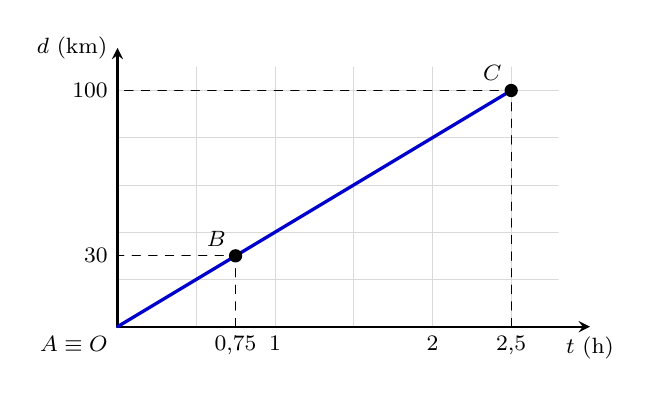
\begin{tikzpicture}[>=stealth, line join=round, line cap=round, font=\footnotesize, xscale=2, yscale=0.03]
	\foreach \y in {20,40,60,80,100} \draw[gray!30, very thin] (0, \y) -- (2.8, \y);
	\foreach \x in {0.5,1,1.5,2,2.5} \draw[gray!30, very thin] (\x, 0) -- (\x, 110);
	\draw[->, thick] (0, 0) -- (3.0, 0) node[below] {$t\text{ (h)}$};
	\draw[->, thick] (0, 0) -- (0, 118) node[left] {$d\text{ (km)}$};
	\draw[very thick, blue!80!black] (0, 0) -- (2.5, 100);
	\draw[dashed] (0.75, 0) -- (0.75, 30) -- (0, 30);
	\draw[dashed] (2.5, 0) -- (2.5, 100) -- (0, 100);
	\fill (0.75, 30) circle (1.2pt and 80pt);
	\fill (2.5, 100) circle (1.2pt and 80pt);
	\node[above left] at (0.75, 30) {$B$};
	\node[above left] at (2.5, 100) {$C$};
	\node[below left] at (0, 0) {$A \equiv O$};
	\foreach \x/\l in {0.75/0{,}75, 2.5/2{,}5, 1/1, 2/2} \node[below] at (\x, 0) {$\l$};
	\foreach \y in {30, 100} \node[left] at (0, \y) {$\y$};
\end{tikzpicture}
\end{document}
